\documentclass[tikz,border=10pt]{standalone}
\usepackage{amsmath}
\usetikzlibrary{arrows.meta, positioning, calc, decorations.pathreplacing}
\definecolor{c1}{HTML}{000000}
\definecolor{c2}{HTML}{233D4D}
\definecolor{c3}{HTML}{FE7F2D}
\definecolor{c4}{HTML}{EAECF0}
\definecolor{axiscolor}{HTML}{333333}
\definecolor{labelcolor}{HTML}{5F6B75}
\begin{document}
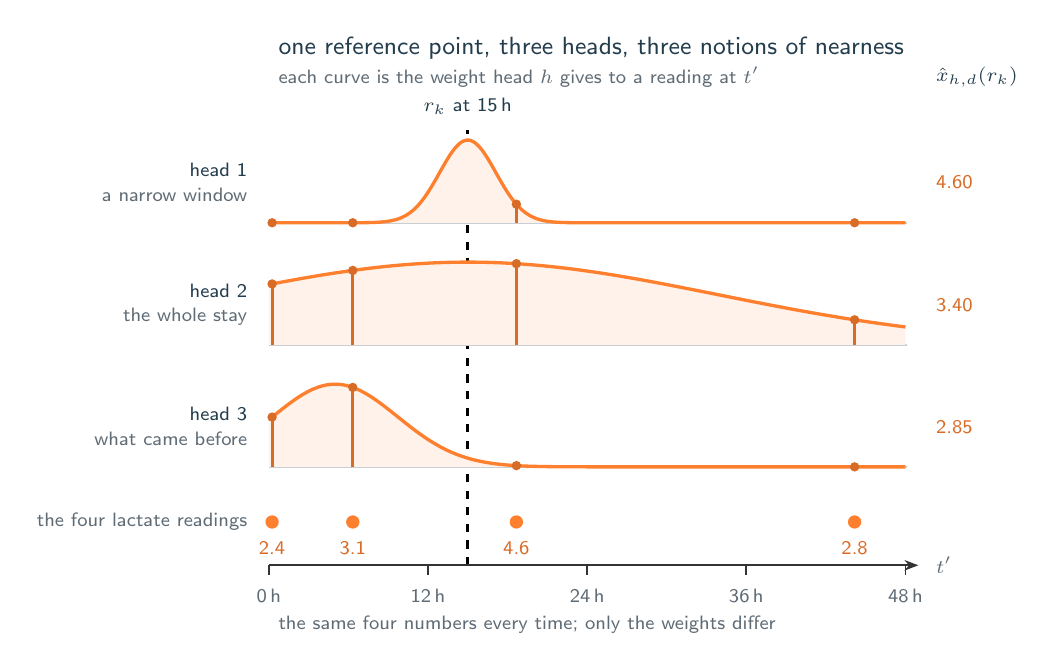
\begin{tikzpicture}[
    every node/.style={font=\sffamily},
    lab/.style={font=\sffamily\scriptsize, text=labelcolor},
    tag/.style={font=\sffamily\scriptsize, text=c2},
    hot/.style={font=\sffamily\scriptsize, text=c3!85!black},
]
\def\X#1{3.10 + #1*0.00280}
\def\A{1.05}

% a gaussian with a clamped exponent, so the plot never underflows
\newcommand{\gauss}[3]{\A*exp(max(-30, -((#1-#2)/#3)*((#1-#2)/#3)))}

% one head: baseline #1, centre #2, width #3
\newcommand{\headrow}[3]{%
  \draw[c2!25, line width=0.7pt] (3.10, #1) -- (11.20, #1);
  \fill[c3!10] plot[domain=0:2880, samples=300, smooth]
      ({\X{\x}}, {#1 + \gauss{\x}{#2}{#3}})
      -- ({\X{2880}}, #1) -- ({\X{0}}, #1) -- cycle;
  \draw[c3, line width=1.2pt] plot[domain=0:2880, samples=300, smooth]
      ({\X{\x}}, {#1 + \gauss{\x}{#2}{#3}});
  \foreach \m in {15, 380, 1120, 2650}{
      \pgfmathsetmacro\hgt{\gauss{\m}{#2}{#3}}
      \draw[c3!85!black, line width=1.1pt] ({\X{\m}}, #1) -- ({\X{\m}}, {#1+\hgt});
      \fill[c3!85!black] ({\X{\m}}, {#1+\hgt}) circle (1.7pt);}}

\node[tag, anchor=west, font=\sffamily\small] at (3.10, 7.52)
     {one reference point, three heads, three notions of nearness};
\node[lab, anchor=west] at (3.10, 7.15)
     {each curve is the weight head $h$ gives to a reading at $t'$};
\node[tag, anchor=west] at (11.45, 7.15) {$\hat{x}_{h,d}(r_k)$};

\draw[c1, line width=0.9pt, dashed] ({\X{900}}, 0.95) -- ({\X{900}}, 6.48);
\node[tag, anchor=south] at ({\X{900}}, 6.55) {$r_k$ at 15\,h};

\headrow{5.30}{900}{180}
\node[tag, anchor=east, align=right] at (2.95, 5.81)
     {head 1\\[1pt] \textcolor{labelcolor}{a narrow window}};
\node[hot, anchor=west] at (11.45, 5.81) {4.60};

\headrow{3.75}{900}{1600}
\node[tag, anchor=east, align=right] at (2.95, 4.26)
     {head 2\\[1pt] \textcolor{labelcolor}{the whole stay}};
\node[hot, anchor=west] at (11.45, 4.26) {3.40};

\headrow{2.20}{300}{400}
\node[tag, anchor=east, align=right] at (2.95, 2.71)
     {head 3\\[1pt] \textcolor{labelcolor}{what came before}};
\node[hot, anchor=west] at (11.45, 2.71) {2.85};

% the record, drawn once
\node[lab, anchor=east] at (2.95, 1.50) {the four lactate readings};
\foreach \m/\v in {15/2.4, 380/3.1, 1120/4.6, 2650/2.8}{
    \fill[c3] ({\X{\m}}, 1.50) circle (2.4pt);
    \node[hot, anchor=north] at ({\X{\m}}, 1.37) {\v};}

\draw[axiscolor, line width=0.8pt, -{Stealth[length=5pt]}] (3.10, 0.95) -- (11.35, 0.95);
\foreach \h in {0, 12, 24, 36, 48}{
    \pgfmathsetmacro\m{\h*60}
    \draw[axiscolor, line width=0.7pt] ({\X{\m}}, 0.95) -- ({\X{\m}}, 0.83);
    \node[lab, anchor=north] at ({\X{\m}}, 0.77) {\h\,h};}
\node[lab, anchor=west] at (11.45, 0.95) {$t'$};

\node[lab, anchor=west] at (3.10, 0.20)
     {the same four numbers every time; only the weights differ};
\end{tikzpicture}
\end{document}
